% Remember to input this to the presentative tex file before compiling.

\section{Basic concepts and definitions of Markov Chain}

\subsection{Definitions}

\begin{frame}
    \begin{definition}[Markov Chain]
        $S$ : state-space(countable set),
        $\theta$ : stochastic variable, \\
         $\{\theta^{(t)} \in S |t=0,1,...\}$
         : discrete time stochastic processes \\
         If $\{\theta^{(t)}\}_t $ satisfies\\
         \[
         P(\theta^{(t+1)} \in A |\theta^{(0)} = x_0,...,\theta^{(t)} =x) 
         = P(\theta^{(t+1)} \in A  |\theta^{(t)} = x)
         \]\\
         \[\forall x,x_{t-1},...,x_{0}\in S, A \subset S, t = 0,1,...\]\\
        then,  $\{\theta^{(t)}\}_t $ is said to be \textbf{Markov Chain}. 
    \end{definition}
    \Large The future states only depend on present states, not on the past states.\\
\end{frame}

\begin{frame}{frame title}
    \begin{definition}[time-homogeneous]
        if $\{\theta^{(t)}\}_t $ satisfies 
        \[
        P(\theta^{(t+1)} \in A  |\theta^{(t)} = x) 
        = P(\theta^{(t+1)} \in A  |\theta^{(t)} = x) := P(x|A), \\ 
        \forall x,x_{t-1},...,x_{0}\in S, A \subset S, t = 0,1,...
        \]\\
        Then, Markov Chain is said to be \textbf{time-homogeneous}.
    \end{definition}
    
    
    \Large States transition probabilities are independent from time, $t$.
\end{frame}

\begin{frame}{Stochastic matrix}
    \begin{definition}
        Define $P(x,y)$ as below.
        \[P(x,y):= P(\theta^{(t+1)} =y  |\theta^{(t)} = x)\]
        
        Then, \textbf{stochastic matrix} $P$ is defined as below.
        \[
        P := 
        \begin{pmatrix}
            P(x_1,x_1) & \cdots & P(x_1,x_r) 
            \\\vdots & \ddots &\vdots        
            \\P(x_r,x_1) & \cdots & P(x_r,x_r)
        \end{pmatrix}
        \]
        
        More generally, A real $r*r$ matrix $P$ is said to be \textbf{stochastic matrix} if and only if its elements are all non-negative and its rows sums to 1.
    \end{definition}
\end{frame}

\subsection{Examples}
\begin{frame}
    \begin{exampleblock}{An example of a naive Markov Chain.}
        \begin{columns}
            \begin{column}{0.7\textwidth}
                Let's look at the situation shown on the right.
                \[P(\theta^{(t+1)} = 1  |\theta^{(t)} = 1) = 0.6\]
                \[P(\theta^{(t+1)} = 1  |\theta^{(t)} = 2) = 0.2\]
                \[P(\theta^{(t+1)} = 2  |\theta^{(t)} = 1) = 0.4\]
                \centerline{\vdots}\\
                Each probability is independent from $t$.\\
                The transition matrix $P$ is below.
                \[P := 
                    \begin{pmatrix}
                        0.6 & 0.4 & 0
                        \\0.2 & 0.3 &0.5       
                        \\0 & 0 & 1
                    \end{pmatrix}\]                
            \end{column}
            \begin{column}{0.25\textwidth}
                \begin{figure}[h]
                 \centering
                 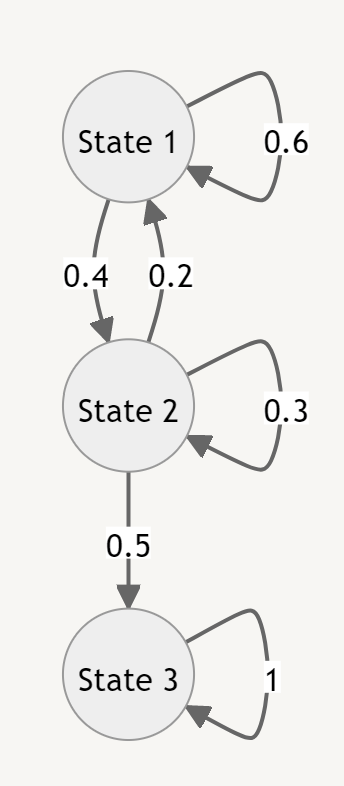
\includegraphics[width=2.0cm]
                      {Images/Figures/states transition figure.png}
                 \caption{図の説明}
                 \label{ラベル名}
                \end{figure}
            \end{column}
        \end{columns}        
    \end{exampleblock}
\end{frame}


\subsection{Lemmas}
\begin{frame}
    \begin{lemma}
        \label{lemmaA} The product of two stochastic matrices is another stochastic matrix.        
    \end{lemma}  
    Proof.\\
    let $P=(p_{ij}) _{ij}, Q = (q_{ij}) _{ij}$ be stochastic matrices. From definition of matrix product, $(PQ)_{ij} = \sum_{k} p_{ik}q_{kj}$ . 
    Also, stochastic matrices satisfies 
    $\forall i\in\mathbb{N},\quad\sum_{j}  p_{ij} = 1,\quad\sum_{j}  q_{ij} = 1$ 
    \[
    \therefore \sum_{j} (PQ)_{ij}
    = \sum_{j} \sum_{k} p_{ik}q_{kj}
    = \sum_{k} \left(p_{ik}\sum_{j}  q_{kj}\right) = \sum_{k} p_{ik} = 1
    \]
    Therefore, sum of  $i$th row of $PQ$ equals to 1, thus $PQ$ is another stochastic matrix.\qed
\end{frame}

\begin{frame}
    \begin{lemma}
        \label{lemmaB} Every eigenvalue $\lambda$ satisfies 
        $|\lambda|\le1$.
    \end{lemma}
    Proof. \\
        Let $P=(p_{ij}) _{ij}$ be stochastic matrices, $v = (v_i)_i$ be eigenvector of $P$, and $\lambda$ be eigenvalue.
        Also, define $m$ as below.
        $$
        m = \argmax_{i} \{|v_1|,...,|v_n|\} 
        $$
        Then, because $Pv = \lambda v$, 
        \[
        \sum_i p_{mi} v_i = \lambda v_m \\
        \therefore |\lambda |
        = \frac{|\sum_i p_{mi} v_i |}{|v_m|} 
        \le \frac{\sum_i p_{mi} |v_i|}{|v_m|}
        \le \frac{\sum_i p_{mi} |v_m|}{|v_m|}
        = \frac{1\cdot |v_m|}{|v_m|} = 1 \qed
        \]
\end{frame}

\begin{frame}
    \begin{lemma}
        \label{lemmaC} Every stochastic matrix has at least one eigenvalue equal to 1.
    \end{lemma}  
    Proof.\\
    Let $P=(p_{ij}) _{ij}$ be a stochastic matrix, $v_0$ be a vector s.t.$ v_0 = (1,\cdots,1)$, then
    \[
    \forall i, (Pv_0)_i = \sum_j p_{ij} = 1 = (v_0)_i
    \therefore Pv_0 = v_0
    \]
    Thus, $P$ has at least one eigenvalue equal to 1. \qed
\end{frame}